\documentclass{article}
\pdfpagewidth=8.5in
\pdfpageheight=11in

\usepackage{official_template/ijcai26}
\usepackage{times}
\usepackage{xurl}
\usepackage[hidelinks]{hyperref}
\usepackage[utf8]{inputenc}
\usepackage[small]{caption}
\usepackage{graphicx}
\usepackage{amsmath,amssymb}
\usepackage{booktabs}
\usepackage{array}
\usepackage{microtype}
\usepackage{tikz}
\usetikzlibrary{arrows.meta,positioning,fit,backgrounds,shapes.geometric,calc}

\urlstyle{same}
\pdfinfo{/TemplateVersion (IJCAI.2026.0)}

\definecolor{inputblue}{RGB}{225,238,248}
\definecolor{modelviolet}{RGB}{239,229,247}
\definecolor{guardorange}{RGB}{252,235,215}
\definecolor{runtimegreen}{RGB}{224,242,231}
\definecolor{ledgergray}{RGB}{239,241,244}
\definecolor{rejectred}{RGB}{249,229,229}
\newcolumntype{L}[1]{>{\raggedright\arraybackslash}p{#1}}
\newcolumntype{C}[1]{>{\centering\arraybackslash}p{#1}}

\title{PACT: Evidence-Bound Planning for\
Contract-Governed Tool Agents}

\author{
Pu Yang$^1$\And
Feng Ye$^2$\\
\affiliations
$^1$Huawei Canada, Edison Research Center\\
$^2$University of Victoria\\
\emails
npuyangpu@gmail.com, fengye@uvic.ca
}

\begin{document}
\maketitle

\begin{abstract}
Tool-using language agents must interpret underspecified requests while
respecting mutable capability contracts and avoiding unsupported claims of
success.  We present PACT, a CAR-bench Track~2 agent that restricts its
Cerebras-hosted language model to semantic proposal.  The model compiles the
current policy, request, capabilities, and evidence into a bounded obligation
graph; a deterministic kernel alone may release the next user interaction or
tool call.  Before release, the kernel strictly decodes the graph, validates
its structure and arguments against live Draft~2020--12 schemas, and enforces
capability freshness, one-shot confirmation scopes, and terminal evidence
requirements.  PACT recompiles when an event introduces a new semantic
binding; otherwise a control-only event advances an immutable verified suffix.
Every Act result reported as successful remains a completion obligation across
later horizons.  Each horizon uses one proposal, at most one verifier-guided
repair, and, for action-bearing plans, one separate same-model audit.  We state
conditional guarantees for capability confinement, scoped confirmation, and
evidence-closed completion; language interpretation remains outside the
assurance boundary.  Failure-oriented tests exercise rejection, contract drift,
event mismatch, scope reuse, and carried-obligation violations; digest-pinned
A2A validation establishes packaging and telemetry, not task quality.
\end{abstract}

\section{Introduction}

CAR-bench exposes brittle control through multi-turn state changes, missing
capabilities, and ambiguous requests \cite{kirmayr2026car}.  Its A2A evaluator
sends policy, conversation, live tool declarations, and tool results
\cite{a2a2026}; the agent selects the next interaction, while the evaluator
executes tools.  Track~2 additionally audits sequential model-call depth and
token telemetry.

The reliability problem is one of authority.  A conventional reason--act loop
lets one stochastic component interpret the request, construct arguments,
accept confirmation, and declare completion.  Valid JSON constrains syntax but
does not show that an operation remains live, that its arguments satisfy the
current schema, or that a result justifies completion.

PACT separates semantic flexibility from execution authority.  The model
proposes a short obligation graph; deterministic code admits and advances it
only after checking live contracts, dependencies, confirmation, and evidence.
An Observe result or Ask reply is a semantic \emph{data event} and starts a new
horizon.  An exact confirmation or matched Act success is a \emph{control
event} and advances the verified suffix without another model call.  Every Act
record reported as successful remains mandatory completion evidence across
later horizons.

\paragraph{Contributions.}
PACT makes two methodological contributions.  First, \emph{verified-horizon
execution} lets events that only discharge a checked obligation advance an
immutable suffix, while events that may change an operation, argument, or scope
invalidate the horizon and re-enter compilation.  Second, \emph{cross-horizon
completion closure} keeps every reported-success Act record mandatory for any
later \texttt{completed} outcome.  The implementation additionally exposes a
bounded serial inference graph (Figure~\ref{fig:architecture}) and a
deterministic validation suite.  The kernel contains no task IDs, benchmark
utterances, operation allowlists, or domain workflows.

\section{Related Work and Positioning}

ReAct interleaves model reasoning and acting \cite{yao2023react}.
LLMCompiler optimizes parallel function dispatch \cite{kim2024llmcompiler};
PlanCompiler validates typed pipelines over a fixed primitive registry
\cite{harikumar2026plancompiler}; and AgentSpec externalizes runtime rules
\cite{wang2026agentspec}.  As scoped here, none couples a revocable,
per-emission capability contract to terminal evidence carried across planning
horizons.  PACT instead serializes visible obligations, binds A2A transitions
to reported outcomes, and revalidates the live contract before release.

The producer/checker split is inspired by proof-carrying code
\cite{necula1997pcc} and runtime verification \cite{leucker2009runtime}, but
PlanIR is a locally checked execution artifact, not a proof of language meaning.

\begin{figure*}[t]
\centering
\resizebox{0.985\textwidth}{!}{%
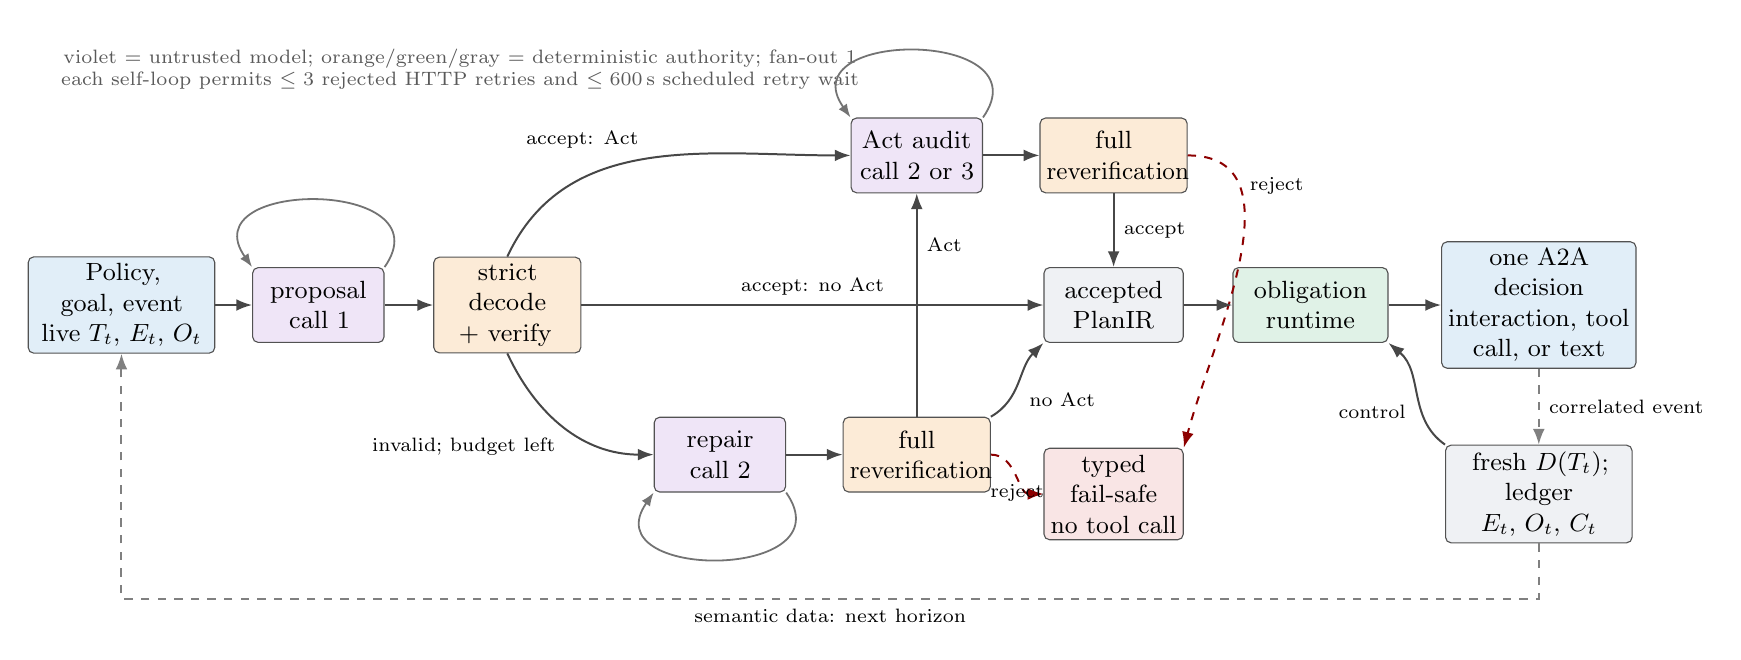
\begin{tikzpicture}[
  x=1mm, y=1mm,
  box/.style={draw=black!68, rounded corners=2pt, align=center,
              minimum height=9.5mm, text width=18mm, inner sep=2.4pt,
              font=\small},
  model/.style={box, fill=modelviolet},
  guard/.style={box, fill=guardorange},
  runtime/.style={box, fill=runtimegreen},
  state/.style={box, fill=ledgergray},
  input/.style={box, fill=inputblue},
  reject/.style={box, fill=rejectred, text width=16mm},
  arrow/.style={-{Latex[length=2.0mm]}, line width=.72pt, draw=black!72},
  feedback/.style={arrow, dashed, draw=black!50},
  rejectarrow/.style={arrow, dashed, draw=red!55!black},
  retry/.style={-{Latex[length=1.7mm]}, line width=.65pt, draw=black!55}
]
\node[input, text width=22mm] (input) at (0,0)
  {Policy, goal, event\\live $T_t$, $E_t$, $O_t$};
\node[model, text width=15mm] (proposal) at (25,0)
  {proposal\\call 1};
\node[guard, text width=17mm] (verify) at (49,0)
  {strict decode\\+ verify};
\node[model, text width=15mm] (repair) at (76,-19)
  {repair\\call 2};
\node[guard, text width=17mm] (repairverify) at (101,-19)
  {full\\reverification};
\node[model, text width=15mm] (audit) at (101,19)
  {Act audit\\call 2 or 3};
\node[guard, text width=17mm] (auditverify) at (126,19)
  {full\\reverification};
\node[state, text width=16mm] (plan) at (126,0)
  {accepted\\PlanIR};
\node[runtime, text width=18mm] (runtime) at (151,0)
  {obligation\\runtime};
\node[input, text width=23mm] (a2a) at (180,0)
  {one A2A decision\\interaction, tool call, or text};
\node[reject] (safe) at (126,-24)
  {typed fail-safe\\no tool call};
\node[state, text width=22mm] (state) at (180,-24)
  {fresh $D(T_t)$; ledger\\$E_t$, $O_t$, $C_t$};
\node[font=\scriptsize, text=black!65, align=center] at (43,30)
  {violet = untrusted model; orange/green/gray = deterministic authority;
   fan-out 1\\
   each self-loop permits $\leq3$ rejected HTTP retries and
   $\leq600$\,s scheduled retry wait};

\draw[arrow] (input) -- (proposal);
\draw[arrow] (proposal) -- (verify);
\draw[arrow] (verify) -- node[above, font=\scriptsize]{accept: no Act} (plan);
\draw[arrow] (verify.north) to[out=65,in=180]
  node[above left, font=\scriptsize]{accept: Act} (audit.west);
\draw[arrow] (audit) -- (auditverify);
\draw[arrow] (auditverify.south) -- node[right, font=\scriptsize]{accept}
  (plan.north);
\draw[arrow] (verify.south) to[out=-65,in=180]
  node[below left, font=\scriptsize]{invalid; budget left} (repair.west);
\draw[arrow] (repair) -- (repairverify);
\draw[arrow] (repairverify.north east) to[out=30,in=-135]
  node[below right, font=\scriptsize]{no Act} (plan.south west);
\draw[arrow] (repairverify.north) --
  node[right, pos=.77, font=\scriptsize]{Act} (audit.south);
\draw[rejectarrow] (repairverify.east) to[out=0,in=180]
  node[below, font=\scriptsize]{reject} (safe.west);
\draw[rejectarrow] (auditverify.east) to[out=0,in=75]
  node[right, near start, font=\scriptsize]{reject} (safe.north east);

\draw[arrow] (plan) -- (runtime);
\draw[arrow] (runtime) -- (a2a);
\draw[feedback] (a2a) -- node[right, font=\scriptsize]{correlated event} (state);
\draw[arrow] (state.north west) to[out=145,in=-40]
  node[below left, font=\scriptsize]{control} (runtime.south east);
\draw[feedback] (state.south) -- ++(0,-7) -|
  node[below, near start, font=\scriptsize]{semantic data: next horizon}
  (input.south);

\draw[retry] (proposal.north east) to[out=55,in=125,looseness=2.1]
  (proposal.north west);
\draw[retry] (repair.south east) to[out=-55,in=-125,looseness=2.1]
  (repair.south west);
\draw[retry] (audit.north east) to[out=55,in=125,looseness=2.1]
  (audit.north west);
\end{tikzpicture}}
\caption{One Track~2 decision horizon, corresponding to a baseline LLM step.
The maximum completed-model path is proposal $\rightarrow$ repair
$\rightarrow$ Act audit: three serial calls.  The audit is used only for an
accepted Act plan, and its replacement is fully reverified.  A rate-limited
transport attempt yields no completion or tokens; exhaustion fails safely.
Ask/Observe data start a new horizon, whereas exact confirmation and matched
Act success advance the immutable suffix.}
\label{fig:architecture}
\end{figure*}

\section{PACT}

\subsection{Trust Model and State}

PACT trusts its sole-emission adapter, PlanIR/schema validators, digest checks, and
evaluator policy/capability metadata.  Result values remain
untrusted semantic data, but the claims assume that the evaluator
returns the result of the sole pending call and truthfully reports its explicit
\texttt{SUCCESS}/\texttt{FAILURE} status.  PACT validates the envelope and
local binding; it does not independently attest the external effect.  A2A
supplies an evaluator call ID but echoes no agent-selected nonce.

For each active goal, the adapter stores the live contract $T_t$, an append-only
evidence ledger $E_t$, the accepted graph $G_t$, at most one waiting runtime
obligation $p_t$, reported-success Act-key obligations $O_t$, consumed
confirmation scopes $C_t$, and accumulated inference metrics $M_t$.  Values cross the
ledger through a JSON round trip, preventing caller mutation of nested history.
Event fingerprints make identical replay idempotent; conflicting reuse and
out-of-order input cannot satisfy a waiting node.  Per-context locks serialize
turns, and cancellation deletes goal state without replacing its lock.

\subsection{Compile, Verify, and Audit}

The semantic compiler receives the trusted policy in a separate system
partition and a bounded view of the goal, recent events, $T_t$, $E_t$, and
$O_t$.  Its provider-facing language is deliberately smaller than PlanIR.
Because Cerebras strict response schemas forbid unconstrained object
properties \cite{cerebras2026structured}, operation arguments travel as one
\texttt{arguments\_json} string.  The local decoder rejects duplicate keys and
non-finite numbers, decodes exactly one JSON object, and validates it against
the live Draft~2020--12 operation schema \cite{jsonschema2020}.  Provider
constrained decoding is therefore an early filter, not the authority; empirical
structured-generation work motivates retaining this local check
\cite{geng2025structured}.

PlanIR is a bounded DAG over
\[
 \{\textsc{Observe},\textsc{Ask},\textsc{Confirm},
   \textsc{Act},\textsc{Respond}\}.
\]
\textsc{Observe} and \textsc{Act} identify a live operation, constant
arguments, and a fresh success-evidence key.  \textsc{Ask} and
\textsc{Confirm} wait for a user event; each \textsc{Confirm} explicitly names
the descendant Act nodes it authorizes.  The sole terminal
\textsc{Respond} has one of five outcomes: \texttt{completed},
\texttt{answered}, \texttt{refused}, \texttt{declined}, or
\texttt{fail\_safe}.  The verifier checks unique identifiers, existing
dependencies, acyclicity, terminal reachability, at most 20 nodes, dependency
depth at most 12, evidence freshness, operation membership, and the complete
recursive argument schema.

One rejected proposal may be repaired from value-redacted typed issues.  A
second rejection fails safely.  After a plan containing an Act node passes
locally, a separate same-model prompt audits the full policy, goal, evidence,
capabilities, and argument provenance.  The audit returns a complete
replacement candidate, which crosses the entire decoder and verifier again;
failure never falls back to the pre-audit plan.  This pass is a stochastic
cross-check, not a semantic proof.  The submitted default is
\texttt{gpt-oss-120b}, medium reasoning, and 8,192 maximum completion tokens.
A provider \texttt{length} finish is a typed truncation and does not trigger a
futile identical semantic repair.

\subsection{Execute, Replan, and Close Evidence}

The runtime deterministically chooses the first topologically ready node,
emits one runtime obligation, and waits.  Before an external Observe or Act
call, it rebuilds the complete capability snapshot, requires an unchanged
digest, rechecks operation membership and any known effect label, and validates
a deep-copied argument object again.  A revoked or changed contract therefore
cannot inherit admission from an older snapshot.

\paragraph{Verified-horizon principle.}
An event is \emph{control-only} when it supplies no value that can parameterize
an unexecuted node and merely discharges the unique waiting obligation.  An
exact positive confirmation and a reported-success Act result whose
continuation depends only on status are control-only: PlanIR has constant
arguments and no expression language, so neither event can rewrite the
accepted suffix.  If $G_t$ was verified under digest $d$, the event matches
$p_t$, and the live digest remains $d$, processing changes only node status and
the prescribed ledger, $O_t$, or $C_t$ record.  Names, arguments,
dependencies, and remaining order are unchanged, so the next ready node may be
released without semantic recompilation, subject to the emission guard.

Ask replies, Observe results, and qualified confirmations instead introduce a
value or scope with no verified binding in the old graph.  PACT discards that
horizon, preserves $E_t$ and $O_t$, and recompiles.  This data/control cut is a
validity boundary, not a latency heuristic.  It preserves checked structure
and evidence obligations, not semantic correctness.  Each reported-success Act
key enters $O_t$, so later replanning cannot silently forget it.

The adapter accepts exactly one external result, requires the pending operation
name and a nonempty evaluator call ID, then binds the payload to the sole
pending context, plan, node, argument digest, and capability digest.  The
runtime validates this internally bound event.  Correlation is therefore
unambiguous under the single-pending assumption but is not independently
authenticated by echoed metadata.  Only an explicit reported
\texttt{SUCCESS} creates successful external evidence.  Local lowering
replaces model-proposed completion citations with the current Act keys plus
$O_t$ and checks their producers and status.  An \texttt{answered} outcome
contains no Act node; semantic effect coverage requires trusted effect metadata.

Confirmation is required only when trusted metadata sets
\path{x-pact-requires-confirmation} or the trusted description begins with the
anchored marker \path{REQUIRES_CONFIRMATION}.  A qualifying authorization is
either a same-plan ancestor or an unused ledger scope
\begin{equation}
 \bigl(D(T_t),\,o,\,\operatorname{SHA256}(x)\bigr),
 \label{eq:scope}
\end{equation}
where $D(T_t)$ is the digest of the entire capability snapshot, $o$ the
operation, and $x$ its canonical arguments.  A matching successful Act consumes
only its individual scope.  Using the full snapshot is conservative: even an
unrelated capability change invalidates prior authorization.

\section{Enforced Properties and Compute}

Table~\ref{tab:guarantees} separates locally enforced properties from their
assumptions.  Three invariants carry the main argument.  First, if PACT emits
tool call $(o,x)$, then $o\in T_t$, $x\models
\operatorname{schema}_{T_t}(o)$, and the current snapshot digest equals the
admission digest.  This follows because admission and the sole emission path
perform the same membership and schema checks.

Second, let $\mathcal{K}_{A}(E)$ be the evidence keys in $E$ whose source is
external, producer is \textsc{Act}, and explicit status is \texttt{success}.
\begin{equation}
\texttt{completed}\ \Longrightarrow\
\operatorname{ActKeys}(G_t)\cup O_t\subseteq\mathcal{K}_{A}(E_t).
\end{equation}
Unmatched, failed, duplicated, or conflicting events cannot satisfy a waiting
node.  Current keys originate at Act producers; carried keys must resolve to
reported-success external Act records.  Induction over horizons establishes
obligation monotonicity: a reported-success Act adds one key to $O_t$, and no
nonterminal replan removes it.

Third, confirmation requires a same-plan ancestor or unused scope from
Equation~\ref{eq:scope}; success consumes that scope and $C_t$ prevents reuse.

\begin{table}[t]
\centering
\footnotesize
\setlength{\tabcolsep}{3pt}
\begin{tabular}{@{}L{.22\columnwidth}L{.70\columnwidth}@{}}
\toprule
Property & Enforcement and assurance boundary\\
\midrule
Call confinement &
Live membership and full Draft~2020--12 argument validation at admission and
emission under one digest; assumes the evaluator's declaration accurately
describes the operation.\\
Transition integrity &
One waiting obligation; operation and nonempty evaluator-ID checks followed by
internal binding/validation.  A2A provides no echoed agent nonce.\\
Scoped confirmation &
Same-plan ancestry or unused $(D(T_t),o,\operatorname{SHA256}(x))$ scope;
individual consumption after Act success.  Requires trusted metadata and
confirmation parsing that reflects intended consent.\\
Completion closure &
Reported-success Act evidence plus all carried keys.  Real effect coverage
requires truthful status and trusted effect metadata.\\
Compute audit &
Depth at most three and fan-out one; transport attempts, tokens, and
normally-returned-call quota wait are separated.\\
\bottomrule
\end{tabular}
\caption{The assurance boundary: what code enforces and what remains an
environmental or semantic assumption.}
\label{tab:guarantees}
\end{table}

\paragraph{Track~2 compute audit.}
Horizon $j$ replaces one baseline-agent LLM call.  With
$r_j,a_j\in\{0,1\}$ indicating repair and Act audit, its completed depth is
\begin{equation}
 L_j=1+r_j+a_j\leq3\leq5,
 \label{eq:calls}
\end{equation}
with fan-out one: no-Act branches use one or two completions and Act branches
two or three.  Each invocation permits one initial HTTP request plus at most
three rate-limit retries, hence at most 12 attempts and 1,800 seconds of
scheduled rate-limit wait per horizon.  A rate-limited attempt returns no model
completion or tokens; exhaustion raises a typed error.

Cerebras reports reasoning inside provider completion tokens.  PACT therefore
exports \texttt{prompt\_tokens} as input tokens,
\texttt{thinking\_tokens} as reasoning tokens, and
\texttt{completion\_tokens} as provider completion minus reasoning.  These
fields are mutually exclusive and accumulate across rejected proposals,
repair, audit, and tool turns until the next text response.  For $N$ tasks and
their reported-response sets $R_k$, let $p_r,h_r,c_r$ denote input, reasoning,
and non-reasoning completion tokens.  Then
\(
 U_k=\sum_{r\in R_k}(p_r+h_r+c_r)
\),
and Track~2 requires $N^{-1}\sum_k U_k\leq500{,}000$
\cite{carbench2026tracks}.  PACT reports the counters but, for an open
conversation, does not prove this inequality or global termination.
\texttt{avg\_llm\_call\_time\_ms} averages successful SDK-request duration;
\texttt{quota\_wait\_time\_ms} sums quota-eligible wait only for normally
returned invocations.  Wait accumulated by a retry-exhausted invocation is
absent from final telemetry.  Neither metric is end-to-end A2A latency.

\section{Release Validation}

We validate mechanisms and the submitted artifact, not hidden outcomes.
Table~\ref{tab:validation} summarizes failure-oriented coverage.

\begin{table}[t]
\centering
\footnotesize
\setlength{\tabcolsep}{3pt}
\begin{tabular}{@{}L{.24\columnwidth}L{.68\columnwidth}@{}}
\toprule
Mechanism & Adversarial coverage $\rightarrow$ release behavior\\
\midrule
Plan admission &
Duplicate IDs/keys, cycles, excessive depth, unreachable terminals, malformed
wire JSON, exhausted repair, and rejected audit $\rightarrow$ no admission or
tool call.\\
Live contracts &
Nested schemas, combinators, additional properties, malformed declarations,
effect-label mismatch, and revocation $\rightarrow$ local validation, replan,
or emission-time rejection.\\
Event provenance &
Failure, replay, conflicting event ID, wrong operation/digest, out-of-order
result, and caller mutation $\rightarrow$ no success or state advance.\\
Consent and closure &
Stale/reused scope, changed arguments, later failure/replan $\rightarrow$
per-scope consumption and prior Act keys remain mandatory.\\
Compute and protocol &
Truncation, bounded 429s, cancellation, concurrency, and telemetry
$\rightarrow$ bounded semantic/retry paths, serialized context, and typed
exhaustion.\\
\bottomrule
\end{tabular}
\caption{Mechanism-validation matrix for the final configuration.  These tests
establish executable guard behavior, not CAR-bench reward or Pass$^3$.}
\label{tab:validation}
\end{table}

At report freeze on 23 July 2026, \texttt{uv run pytest -q} passed 356 tests
and three subtests.  Ruff passed the full tree, and mypy passed the 18-file
release closure.

\subsection{Failure Semantics and Validation Oracle}

PACT treats failure as an absence of execution authority, rather than merely
as negative text.  Admission or audit rejection and provider-budget exhaustion
create no runtime and release no external call.  Contract invalidation discards
$G_t$ and recompiles with $E_t$ and $O_t$ unchanged; any later outcome passes
the ordinary completion guard.  A mismatched, replayed, conflicting, or
out-of-order event cannot satisfy $p_t$.  Negative confirmation and explicit
external failure terminate the suffix without a new Act.  No failure path
falls back to an unaudited candidate or invents compensation.  Set
$\Delta_t^A=\mathcal{K}_{A}(E_{t+1})\setminus\mathcal{K}_{A}(E_t)$; let
$S(e_t)=\{\kappa\}$ for a valid, matched Act-\texttt{SUCCESS} event carrying
key $\kappa$, and $S(e_t)=\varnothing$ otherwise.  Let $y_t$ be the emitted
outcome.  For typed failure $f_t$, the oracle is
\begin{equation}
\Delta_t^A\subseteq S(e_t),\qquad
f_t\Longrightarrow y_t\neq\texttt{completed}.
\label{eq:failure-oracle}
\end{equation}
This permits a valid Act success before a later closure failure; failure
neither fabricates nor erases one.  Scopes enter $C_t$ only after matching
success.  Partial results are disclosed; no rollback is claimed because a
contract may lack an inverse.

\paragraph{Oracle-driven protocol.}
Positive traces exercise valid advancement; paired negatives alter one
invariant-bearing field---plan ID, operation, argument or capability digest,
event type, or status---and exercise Equation~\ref{eq:failure-oracle}.
Compiler/verifier tests mutate reachability, evidence producers, confirmation
ancestry, and carried obligations before runtime construction.  Cross-horizon
tests try to omit or relabel a carried reported-success Act key.  Confirmation
traces vary arguments, snapshots, and prior consumption; retry tests use a
synthetic clock to reject a sleep before the cumulative budget is exceeded.
Of 356 collected cases, 192 directly target the PACT kernel and 52 cover A2A
response/scenario contracts; the remainder are not claimed as kernel evidence.
These finite traces witness implemented guards, not exhaustiveness over all
event sequences.  They establish mechanism conformance; digest-pinned A2A
smoke establishes deployability.  Neither estimates planning quality, audit
efficacy, CAR-bench reward, or Pass$^3$.

\paragraph{Necessity stress trace.}
Consider a plan admitted under digest $d_0$, authorization for
$(o,x,d_0)$, a reported-success Act, and a later replan that omits its key.
Admission-only schema checking cannot stop release after the contract changes
to $d_1$; a conversation-level confirmation flag can authorize changed
arguments or snapshot; and a terminal check limited to the newest graph can
forget the earlier Act.  PACT assigns these failures to emission-digest
equality, an exact one-shot scope, and $O_t$ closure, respectively.  PlanIR is
therefore a short-lived, contract-bound execution certificate, while ledger
obligations carry commitments across horizons.

\paragraph{Reproducible release identity.}
The public unprivileged \texttt{linux/amd64} image was built from source
revision \url{3255c9320bfa36e3fe0c4647ffc401b78e7259a6} and pinned as
\url{sha256:173fd630e1691b40af55e731e82023c1df9cfcae52d3b84420c1d307eccea6d1}.
An anonymous registry resolution succeeded.  README Option C pulled this exact
digest, received HTTP~200 from both Agent Cards, and all three public-format
harness projections terminated at the A2A boundary with client exit code zero.
It verified \texttt{turn\_metrics} on nine final responses; no task success is
inferred.  The result artifact has
SHA-256
\url{55c43af4ec481a39c609554e2ef9fbe4315816d0340bb892f2f6689036115bbf}.
This is packaging, protocol, and telemetry evidence, not a task-quality
estimate.  We report no final-configuration public aggregate, hidden-set score,
or ranking in the deadline version.

\section{Limitations and Conclusion}

PACT narrows execution authority but does not verify language meaning.  Its
same-model audit may reject or replace an Act candidate, but its error-reduction
effect is unmeasured and it is not independent evidence.  With
\texttt{unknown} effect metadata, PACT cannot establish Observe-versus-Act
intent.  An Act result is control-only: the suffix may depend on status, not a
new payload value; such workflows need an explicit observation boundary.  The
scope guarantee begins after deterministic confirmation parsing and does not
prove intended consent.  Single-pending A2A correlation is not cryptographic,
the ledger is process-local, and safe failure may reduce coverage.

Within those boundaries, PACT gives a precise separation: the model proposes
meaning, while deterministic code owns capability admission, evidence-bearing
state transitions, scoped authorization, and the evidence conditions of a
typed terminal outcome.  Combining that boundary with verified-horizon
execution yields a locally checkable, protocol-accounted Track~2 agent without
benchmark-shaped workflows.
The broader implication is that replanning assurance is not a property of a
plan alone, but of a plan, its live contract, and a monotone evidence
projection.  This boundary transfers to other tool domains only when status,
effect, and correlation assumptions are equally explicit.

\clearpage

\bibliographystyle{official_template/named}
\bibliography{references}

\end{document}
